% ch1.tex
% Dieses Werk ist unter einem Creative Commons Namensnennung-Keine kommerzielle Nutzung-Weitergabe 
% unter gleichen Bedingungen 3.0 Deutschland Lizenzvertrag lizenziert. Um die Lizenz anzusehen, gehen Sie bitte 
% zu http://creativecommons.org/licenses/by-nc-sa/3.0/de/ oder schicken Sie einen Brief an 
% Creative Commons, 171 Second Street, Suite 300, San Francisco, California 94105, USA.


%\chapter{Not all snakes will squish you}\label{ch:notallsnakeswillsquishyou}
\chapter{Nicht alle Schlangen beißen}\label{ch:notallsnakeswillsquishyou}

%Chances are you were given this book for your birthday.  Or possibly for Christmas.  Aunty Mildred was going to give you mismatching socks that were two sizes too large (and you wouldn't want to wear when you grew into them anyway).  Instead, she heard someone talking about this printable book, remembered you had one of those computer-thingamabobs that you tried to show her how to use last Christmas (you gave up when she started trying to talk into the mouse), and got them to print another copy.  Just be thankful you didn't get the mouldy old socks.
Vielleicht hast du dieses Buch zu deinem Geburtstag bekommen. Oder möglicherweise zu Weihnachten. Tante Helga wollte dir schon ein Paar Socken schenken, die dir viel zu groß sind (und du nebenbei gar nicht anziehen wollen würdest, wenn du reinwächst). Stattdessen hat Tante Helga von diesem druckbaren Buch gehört und sich entfernt an dieses Ding erinnert, was bei dir daheim steht und sich Computer nennt. Du wolltest es ihr den Computer letztes Weihnachten erklären, hast dann aber aufgegeben, als sie mit der Maus zu reden anfing. Sei einfach dankbar, dass du nicht die muffigen Socken bekommen hast.
%I hope you're not too disappointed that I popped out of the recycled wrapping paper, instead.  A not-quite-so-talkative (okay, not-talking-at-all) book, with an ominous looking title on the front about ``Learning$\ldots$''.
Ich hoffe du bist nicht zu enttäuscht, als ich aus der bunten Geschenksverpackung rausgesprungen bin. Ein nicht ganz so gesprächiges (gut, gar nicht sprechendes) Buch, mit diesem verdächtigen Titel über ``Lernen$\ldots$''.
%But take a moment to think about how I feel.  If you were the character from that novel about wizards that is sitting on the bookshelf in your bedroom, I'd possibly have teeth... or perhaps even eyes.  I might have moving pictures inside me, or be able to make moaning ghostly sounds when you opened my pages.  Instead, I'm printed out on dog-eared A4 sheets of paper, stapled together or perhaps bound in a folder.  How would I know---I don't have eyes.
Aber nimm dir einen Moment Zeit und überlege wie ich mich fühle. Wenn du der Zauberer aus dem Geschichtenbuch wärst, hätte ich vielleicht Zähne... oder sogar Augen. Vielleicht hätte ich bewegende Bilder auf den Seiten, oder könnte gespenstische Geräusche von mir geben, wenn du mich öffnest. Stattdessen bin ich auf gewöhnlichen A4 Seiten gedruckt, habe Eselsohren und bin zusammengestapelt oder in einer Ordner einsortiert. Woher sollte ich das wissen---ich habe ja keine Augen. 
\\
\\
%\emph{I'd give anything for a nice, sharp set of teeth$\ldots$}
\emph{Ich würde alles für ein Paar schöner scharfer Zähne geben$\ldots$}
\\
\\
%However it's not as bad as it sounds.  Even if I can't talk... or bite your fingers when you're not looking... I can tell you a little bit about what makes computers work.  Not the physical stuff, with wires and computer-chips and cables and devices that would, more than likely, electrocute you as soon as you touched them (so don't!!)---but the hidden stuff running around inside those wires and computer-chips and cables and bits, which make computers actually useful.
Aber es ist nicht so schlimm wie es klingt. Auch wenn ich nicht reden kann... oder dir in die Finger beißen, wenn du nicht hinschaust... Ich kann dir ein wenig darüber erzählen, wie Computer funktionieren. Nicht die physikalischen Dinge wie Strom, Kabel und Computerchips, bei denen man wahrscheinlich einen Stromschlag bekommt, wenn man sie anfasst (tu es bitte nicht), sondern die Dinge die Computer eigentlich nützlich machen.

\begin{wrapfigure}{r}{0.5\textwidth}
  \begin{center}
\includegraphics*[width=70mm]{electrocute.eps}
  \end{center}
\end{wrapfigure}

%It's a little like thoughts running around inside your head. If you didn't have thoughts you'd be sitting on the floor of your bedroom, staring vacantly at the door and drooling down the front of your t-shirt. Without \emph{programs}, computers would only be useful as a doorstop---and even then they wouldn't be very useful, because you'd keep tripping over them in the night.  And there's nothing worse than a stubbed toe in the dark.
Es ist ein wenig wie Gedanken, die in deinem Kopf herumschwirren. Wenn du keine Gedanken hättest, würdest du am Boden des Schlafzimmers hocken und abwesend an die Decke starren und das T-Shirt ansabbern. Ohne \emph{Programme} wären Computer nur als Türstopper verwendbar---und sogar das mehr schlecht als recht, weil man dauern in der Nacht darüber stolpern würde. Und es gibt nichts schlimmeres als ein angestoßener blauer Zeh in der Nacht.
\\
\\
%\emph{I'm just a book and even I know that.}
\emph{Ich bin nur ein Buch, aber sogar ich weiß das.}
\\
\\
%Your family may have a Playstation, Xbox or Wii sitting in the lounge---they're not much use without programs (Games) to make them work.  Your DVD player, possibly your fridge and even your car, all have computer programs to make them more helpful than they would be otherwise.  Your DVD player has programs to help it figure out what to play on a DVD; your fridge might have a simple program to make sure it doesn't use too much electricity, but still keep your food cold; your car might have a computer with a program to warn the driver if they're about to bump into something.\\
Deine Familie hat vielleicht eine Playstation, Xbox oder Wii im Wohnzimmer stehen---die werden erst interessant wenn man ein Programm (Spiel) hat. Der DVD Player, vielleicht der Kühlschrank oder sogar euer Auto haben alle Programme damit sie nützlicher werden. Der DVD Player hat ein Programm, damit die DVD richtig abgespielt werden kann; der Kühlschrank damit er Energie spart und trotzdem die Speisen kühl hält; und das Auto könnte ein Computerprogramm haben, das den Fahrer beim Einparken hilft.\\
%If you know how to write computer programs, you can do all sorts of useful things. Perhaps write your own games. Create web pages that actually do stuff, instead of just sitting there looking somewhat colourful.  Being able to program could possibly even help with your homework.\\
Wenn du weißt, wie man Computer Programme schreibt, kannst du alle möglichen nützlichen Dinge damit tun. Vielleicht schreibst du dein eigenes Spiel. Baust Webseiten, die sogar echte Dinge tun anstatt nur bunt auszusehen. Programmieren können kann dir vielleicht bei der Hausübung helfen.
\\
%That said, let's get onto something a bit more interesting.
Genug geredet, gehen wir zu etwas Ineressanterem.

%\section{A Few Words About Language}
\section{Ein paar Worte über Sprachen}

%Just like humans, certainly whales, possibly dolphins, and maybe even parents (although that's debatable), computers have their own language.  Actually, also like humans, they have more than one language.  There are languages covering just about all the letters of the alphabet.  A, B, C, D and E are not only letters, they're also programming languages (which proves that adults have no imagination, and should be made to read either a dictionary or a thesaurus before naming anything).
Genau wie Menschen, mit Sicherheit auch Wale, vielleicht Delphine und vielleicht sogar Eltern (darüber lässt sich streiten), haben Computer eine eigene Sprache. Eigentlich haben sie genau wie Menschen mehrere Sprachen. Da gibt es Sprachen, die das ganze Alphabet abdecken. A, B, C, D und E sind nicht nur Buchstaben, sondern das sind auch Programmiersprachen (was beweist, dass Erwachsene keine Phantasie haben, und sollten ein Wörterbuch oder Synonymwörterbuch lesen müssen, bevor sie irgendwas benennen).

%There are programming languages named after people, named using simple acronyms (the capital letters of a series of words), and just a few named after a TV show.  Oh, and if you add a few pluses and hashes (+, \#) after a couple of those letters I just listed---that's yet another couple of programming languages as well.  Making matters worse, some of the languages are almost the same, and differ only slightly.
Da gibt es progammiersprachen die nach Leuten benannt sind, einfache Akronyme (die ersten Buchstaben von einer Wortfolge) oder nach Fernsehserien benannt sind. Und wenn man ein Plus oder Eine Raute (+, \#) hinten anhängt, hat man noch einige Sprachen. Was die Sache noch schlimmer macht ist, dass sich einige Sprachen fast nicht unterscheiden und nur ein wenig verschieden sind.
\\
\\
%\emph{What did I tell you?  No imagination!}
\emph{Was habe ich dir gesagt? Keine Phantasie!}
\\
\\
%Luckily, many of these languages have fallen into disuse, or vanished completely; but the list of different ways you can `talk' to a computer is still rather worryingly large.  I'm only going to discuss one of them---otherwise we might as well not even get started.
Zum Glück werden viele Sprachen kaum mehr verwendet oder sind ganz verschwunden; aber die Liste der verschiedenen Wege mit einem Computer zu `reden' ist immer noch beunruhigend lang. Ich werde dir nur eine vorstellen---ansonsten würden wir gar nicht anfangen.
\\
%It would be more productive to sit in your bedroom and drool down the front of your t-shirt$\ldots$
Da wäre es produktiver im Schlafzimmer zu sitzen und das T-Shirt anzusabbern$\ldots$

%\section{The Order of Non-venomous\\Constricting Serpentes$\ldots$}
\section{Ungiftige\\Würgeschlagen$\ldots$}

%$\ldots$or Pythons, for short.
$\ldots$kurzgesagt: Python.

%Apart from being a snake, Python\index{Python} is also a programming language.  However, it was not named after a legless reptile; rather it is one of the few programming languages named after a TV show.  Monty Python was a British comedy show popular during the 1970's (and still popular now, actually), which you have to be a certain age to find amusing.  Anyone below the age of about$\ldots$ let's say 12$\ldots$ will wonder what all the fuss is all about\footnote{Except the fish slapping dance.  That's funny no matter how old you are.}.
Abgesehen davon, dass Pythons\index{Python} Schlangen sind, gibt es auch die Programmiersprache Python. Die Sprache wurde aber nicht nach dem beinlosen Reptil benannt, sondern nach einer Fernsehsendung, die in den siebziger Jahren populär war. Monty Python war eine britische Komödie (die heute immer noch populär ist), die man erst in einem bestimmten Alter lustig findet. Kinder unter$\ldots$ sagen wir zwölf Jahren werden sich über die Begeisterung wundern \footnote{außer dem fish slapping Dance. Der ist lustig, egal wie alt man ist.}.

%There are a number of things about Python (the programming language, not the snake, nor the TV show) that make it extremely useful when you're learning to program.  For us, at the moment, the most important reason is that you can start it up and do stuff really quickly.
Es gibt eine Anzahl von Dingen die Pyhton (die Programmiersprache, nicht die Schlange und auch nicht die Fernsehsendung) sehr nützlich machen, wenn man anfängt zu programmieren. Für uns ist der wichtigste Grund fürs erste, dass man sehr schnell Ergebnisse erzielen kann.

%This is the part where you hope Mum, Dad (or whomever is in charge of the computer), has read the part at the beginning of this book labelled ``A Note for Mums and Dads''.
Jetzt kommt der Teil an dem du darauf hoffst, dass sich deine Mutter, Vater (oder wer auch immer den Computer bedient), das Vorwort diese Buches mit dem Titel ``Ein Hinweiß für Eltern'' gelesen hat.

\noindent
%There's a good way to find out if they actually have read it:
Das hier ist ein guter Weg das herauszufinden.

\begin{WINDOWS}
%Click on the Start button at the bottom left of the screen, click on `All Programs' (which has a green triangle next to it), and hopefully in the list of programs you should see `Python 2.5' (or something like it).  Figure~\ref{fig1} shows you what you should be looking for. Click on `Python (command line)' and you should see something like Figure~\ref{fig2}.
Klick auf das Startsymbol unten links auf dem Monitor. Gehe dann auf `alle Programme' (hat ein grünes Dreieck) und in der Liste siehst du hoffentlich `Python 3.1' (oder so was ähnliches). Abbildung~\ref{fig1} zeigt dir wonach du Ausschau halten sollst. Klicke auf `Pyhton (Kommandozeile) und ein Fenster wie in Abbildung~\ref{fig2} geht auf.

\begin{figure}
\begin{center}
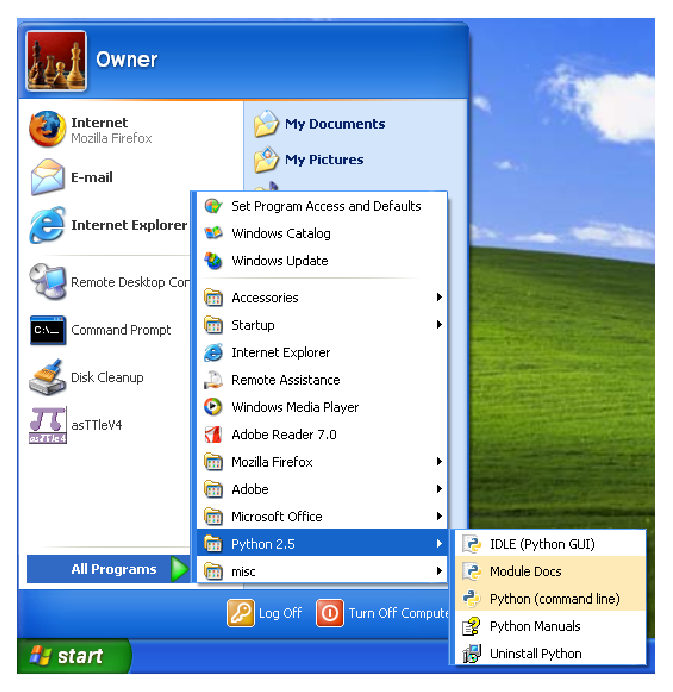
\includegraphics[width=80mm]{figure1.eps}
\end{center}
%\caption{Python in the Windows menu.}\label{fig1}
\caption{Python im Windows Menu.}\label{fig1}
\end{figure}

\begin{figure}
\begin{center}
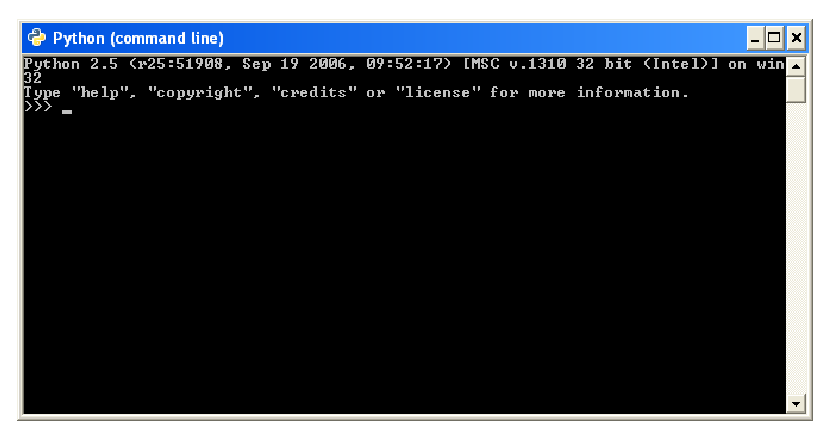
\includegraphics[width=135mm]{figure2.eps}
\end{center}
%\caption{The Python console on Windows.}\label{fig2}
\caption{Die Python console auf Windows.}\label{fig2}
\end{figure}
\end{WINDOWS}

\begin{MAC}
%In Finder, on the left you should see a group called `Applications'.  Click on this, and then find a program called `Terminal' (it'll probably be in a folder called `Utilities').
In der linken Spalte des Finders gibt es die Gruppe `Programme'. Klick einmal drauf und suche nach dem Programm mit dem Namen `Terminal' (es ist wahrscheinlich im Ordner `Dienstprogramme').
%Click on `Terminal', and when it starts up, type python and hit enter.  You'll should hopefully be looking at a window that looks like Figure~\ref{fig3}.
Klicke auf `Terminal' und wenn es sich öffnet tippst du \textbf{python} und drückst die Enter Taste. Du bekommst hoffentlich ein Fenster das so aussieht wie Abbildung~\ref{fig3}.


\begin{figure}
\begin{center}
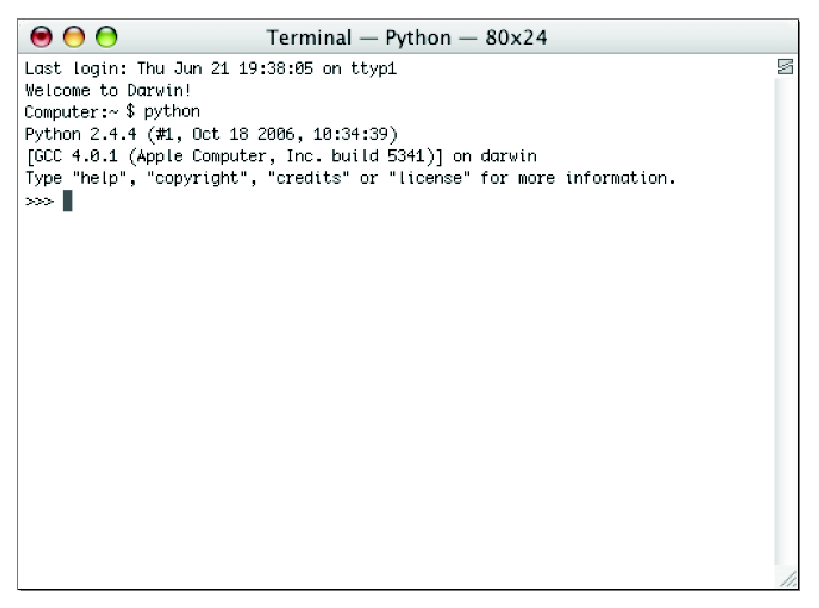
\includegraphics[width=85mm]{figure3.eps}
\end{center}
%\caption{The Python console on Mac OSX.}\label{fig3}
\caption{Die Python console auf Mac OSX.}\label{fig3}
\end{figure}
\end{MAC}

\begin{LINUX}
%Ask Mum or Dad which terminal application you should use (it could be one called `Konsole', `rxvt', `xterm' or any one of a dozen different programs---which is why you'll probably need to ask).  Start the terminal program and type `python' (without the quotes), and hit enter.  You should see something like Figure~\ref{fig4}.
Frage deine Mutter oder deinen Vater welches Terminal Programm du verwenden sollst (es könnte `Konsole', `rxvt', `xterm' oder irgendwie anders heißen---deswegen solltest du wahrscheinlich fragen). Starte das terminal Programm und tippe `python' oder `python3' ein (ohne die Anführungsstriche) und drücke die Eingabetaste. Es sollte etwas wie in Abbildung~\ref{fig4} erscheinen.

\begin{figure}
\begin{center}
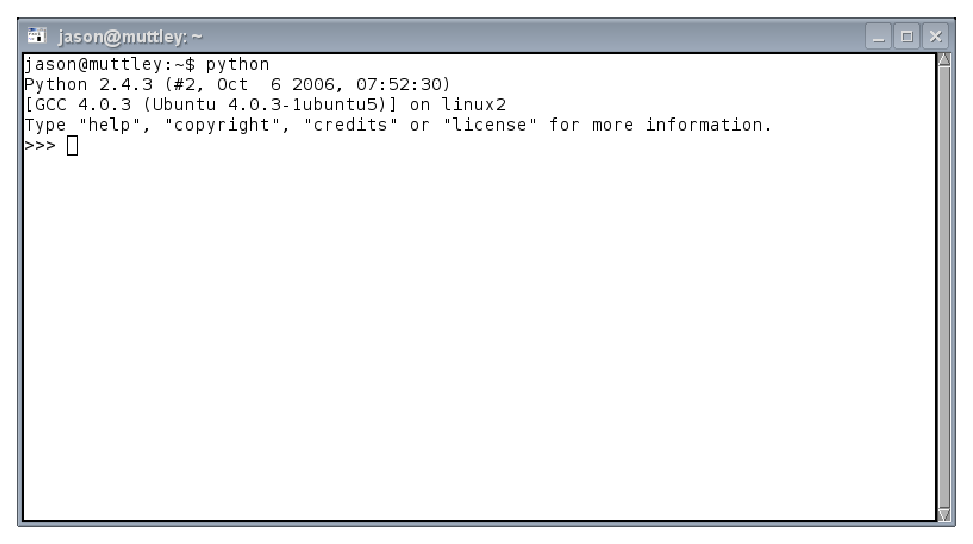
\includegraphics[width=80mm]{figure4.eps}
\end{center}
%\caption{The Python console on Linux.}\label{fig4}
\caption{Die Python console unter Linux.}\label{fig4}
\end{figure}
\end{LINUX}

%\subsection*{\color{BrickRed}If you discover they haven't read the section in the beginning$\ldots$}
\subsection*{\color{BrickRed}Falls du entdeckst hast, dass deine Eltern das Vorwort nicht gelesen haben$\ldots$}

%$\ldots$because there is something missing when you try to follow those instructions---then turn to the front of the book, poke it under their nose while they're trying to read the newspaper, and look hopeful.  Saying, ``please please please please'' over and over again, until it becomes annoying, might work quite well, if you're having trouble convincing them to get off the couch.  Of course, the other thing you can do, is turn to the front of the book, and follow the instructions in the Preface to install Python yourself.
$\ldots$weil irgendetwas nicht mit der vorherigen Anleitung zusammenstimmt---dann blättere zurück und halte deinen Eltern das Buch unter die Nase während sie gerade die Zeitung lesen und schaue sie erwartungsvoll an. Immer wieder ``bitte bitte bitte bitte'' sagen kann dich auch weiterbringen, wenn sie nicht von der Couch aufstehen wollen. Was du immer noch machen kannst ist das Vorwort zu lesen und selber auszuprobieren Python zu installieren.

%\section{Your first Python program}
\section{Dein erstes Python Programm}

%With any luck, if you've reached this point, you've managed to start up the Python console, which is one way of running Python commands and programs.  When you first start the console (or after entering a command), you'll see what's called a `prompt'.  In the Python console\index{Python console}, the prompt is three chevrons, or greater-than symbols ($>$) pointing to the right:
Wenn du mit etwas Glück an dem Punkt angelangt bist und die Python Konsole geöffnet hast, kann es schon losgehen. Wenn die die Konsole das erste Mal öffnest (oder nach dem Ausführen eines Kommandos) siehst du den sogenannten `Promt'. In der Python Konsole\index{Python Konsole}, besteht dieser Prompt aus drei größer-als Zeichen ($>$), die nach rechts zeigen:

\begin{listing}
\begin{verbatim}
>>>
\end{verbatim}
\end{listing}

%If you put enough Python commands together, you have a program that you can run in more than just the console$\ldots$ but for the moment we're going to keep things simple, and type our commands directly in the console, at the prompt ($>>>$).  So, why not start with typing the following:
Wenn du mehrere Python Befehle zusammenbastelst erhältst du ein Programm, welches du auch ausserhalb der Konsole verwenden kannst$\ldots$ aber fürs Erste werden wir die Dinge einfach halten und direkt mit der Konsole nach dem Prompt ($>>>$) arbeiten. Probier es aus und tippe folgendes:

%\begin{listing}
%\begin{verbatim}
%print("Hello World")
%\end{verbatim}
%\end{listing}
\begin{listing}
\begin{verbatim}
print("Hallo Welt")
\end{verbatim}
\end{listing}

%Make sure you include the quotes (that's these: $"$ $"$), and hit enter at the end of the line.  Hopefully you'll see something like the following:
Pass auf, dass du auch die Anführungszeichen verwendest (das sind diese $"$ $"$) und drücke danach die Eingabetaste. Hoffentlich siehst du etwas wie dieses:

%\begin{listing}
%\begin{verbatim}
%>>> print("Hello World")
%Hello World
%\end{verbatim}
%\end{listing}
\begin{listing}
\begin{verbatim}
>>> print("Hallo Welt")
Hallo Welt
\end{verbatim}
\end{listing}

%The prompt reappears, to let you know that the Python console is ready to accept more commands.
Der Prompt erscheint danach wieder um dir zu sagen, dass die Python Konsole wieder bereit für neue Befehle ist.

\noindent
%Congratulations! You've just created your first Python program.  \code{print} is a function that writes whatever is inside the brackets out to the console--we'll use it more later.
Gratulation! Du hast gerade dein erstes Python programm geschrieben. \code{print} ist eine Funktion, die alles innerhalb der Klammern auf die Konsole ausgibt--wir werden das noch öfter verwenden.

%\section{Your Second Python program$\ldots$the same again?}
\section{Dein zweites Python Programm$\ldots$schon wieder das gleiche?}

%Python programs wouldn't be all that useful if you had to type the commands every single time you wanted to do something---or if you wrote a program for someone, and they had to type it in before they could use it.
Python programme wären nicht besonders nützlich, wenn du jedesmal, wenn du etwas tun willst---oder ein Programm für jemanden schreiben willst, alles neu eintippen müsstest.

%The Word Processor that you might be using to write your school assignments, is probably somewhere between 10 and 100 million lines of code.  Depending upon how many lines you printed on one page (and whether or not you printed on both sides of the paper), this could be around 400,000 printed pages$\ldots$ or a stack of paper about 40 metres high.
Das Textverarbeitungsprogramm mit dem du vielleicht deine Hausaufgaben schreibst ist vielleicht zwischen 10 und 100 Millionen Zeilen lang. Abhängig davon wieviele Zeilen du auf ein Blatt druckst (und ob du beidseitig druckst oder nicht) wären das ungefähr 400.000 gedruckte Seiten$\ldots$ oder ein 40 Meter hoher Stapel.
%Just imagine when you brought that software home from the shop, there would be quite a few trips back and forth to the car, to carry that much paper$\ldots$
Stell dir vor, dass du die Software so vom Laden nach Hause bringen würdest. Da müsstest du einige Male hin und her laufen um das ganze Papier nach Hause zu bringen.

%$\ldots$and you'd better hope there's no big gust of wind while you're carrying those stacks. Luckily, there's an alternative to all this typing---or no one would get anything done.
$\ldots$und es wäre besser wenn überhaupt kein Winde weht, während du das Papier nach Hause schleppst. Zum Glück gibt es eine Alternative---sonst würde niemand etwas sinnvolles erreichen.


\begin{center}
\includegraphics*[width=85mm]{pullinghair.eps}
\end{center}

\begin{WINDOWS}
%Open Notepad (Click on Start, All Programs, and it should be in the Accessories sub menu), and then type the print command exactly as you typed it into the console before:
Öffene Notpad (Klicke auf Start, Alle Programme und unter Zubehör sollte Notepad sein), und gib dann das gleiche in die Textdatei ein wie vorher in der Konsole:

%\begin{listing}
%\begin{verbatim}
%print("Hello World")
%\end{verbatim}
%\end{listing}
\begin{listing}
\begin{verbatim}
print("Hallo Welt")
\end{verbatim}
\end{listing}

%Click on the File menu (in Notepad), then Save, and when prompted for a file name, call it \emph{hello.py} and save it on your Desktop. Double-click on the icon for hello.py on your Desktop (see Figure~\ref{fig5}) and for a brief moment a console window will appear.  It will vanish too quickly for you too make out the words, but Hello World will have been printed to the screen for a fraction of a second---we'll come back to this later and prove that it did.\\
Danach einfach im Datei Menu (in Notepad) auf Speichern gehen und wenn nach dem Dateinamen gefragt wird, \emph{hello.py} benennen und auf dem Desktop speichern. Wenn du nun auf dem Desktop Symbol hello.py doppelklickst (siehe Abbildung~\ref{fig5}) wird für einen kurzen Moment die Konsole erscheinen und wieder verschwinden. Es wird zu schnell verschwinden, als die Wörter zu erkennen, aber die Wörter Hallo Welt wird auf dem Monitor für den Bruchteil einer Sekunde erschienen sein---wir kommen nochmals auf das zurück und beweisen, dass es wirklich so ist.\\

\begin{figure}
\begin{center}
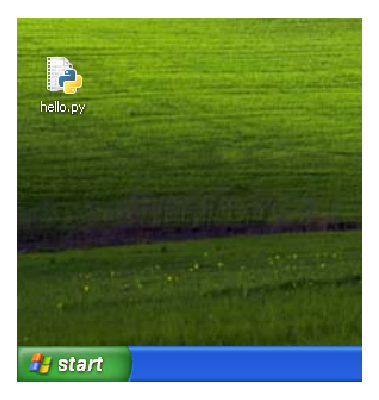
\includegraphics[width=58mm]{figure5.eps}
\end{center}
%\caption{hello.py icon on the Windows Desktop.}\label{fig5}
\caption{hello.py Symbol auf dem Windows Desktop.}\label{fig5}
\end{figure}
\end{WINDOWS}

\begin{MAC}
%Open up the Text Editor by clicking on its icon.  It may be in the Dock at the bottom of the screen \includegraphics*[width=12mm]{textedit-icon.eps}, or look for this icon \includegraphics*[width=19mm]{textedit-icon2.eps} in the Applications list in Finder.  Type the print command exactly as you typed it into the console earlier:
Öffne den Texteditor indem du auf das Symbol klickst. Es ist vielleicht im Dock auf der Unterseite des Monitors \includegraphics*[width=12mm]{textedit-icon.eps}, oder halte nach diesem Symbol \includegraphics*[width=19mm]{textedit-icon2.eps} im Programme Ordner Ausschau. Tippe den print Befehl genau gleich ein, wie du ihn vorher in der Konsole eingegeben hast:

\begin{listing}
\begin{verbatim}
print("Hello World")
\end{verbatim}
\end{listing}
\begin{listing}
\begin{verbatim}
print("Hallo Welt")
\end{verbatim}
\end{listing}

%Click on the File menu, then click on Save, and when you are prompted for a file name, call it hello.py and save it into your home directory (your home directory is on the left under Places--ask Mum or Dad to point it out for you).
Klicke ins Datei Menu und gehe auf Speichern. Gib als Name hello.py ein und speichere es im Home Verzeichnis---frage deine Mutter oder deinen Vater es dir zu zeigen.

%Open the `Terminal' application again--it will automatically start up in your home directory--and type the following:
Öffne danach wieder das `Terminal'--es wird automatisch in deinem Home Verzeichnis starten--und tippe folgendes ein:

\begin{listing}
\begin{verbatim}
python hello.py
\end{verbatim}
\end{listing}

%You should see Hello World written to the window exactly as it was when you typed the command in the Python console.
Du solltest das gleiche Ergebnis in diesem Fenster sehen, wie als du den print Befehl direkt in der Python Konsole eingegeben hast.

\end{MAC}

\begin{LINUX}
%Open a text editor (again you might have to ask Mum or Dad which one to use), then type the print command exactly as you typed it into the console:
Öffne den Texteditor (hier musst du vielleicht deine Eltern fragen, welchen du verwenden sollst), und tippe danach den print Befehl genau gleich ein wie vorher in der Python Konsole:

%\begin{listing}
%\begin{verbatim}
%print("Hello World")
%\end{verbatim}
%\end{listing}
\begin{listing}
\begin{verbatim}
print("Hallo Welt")
\end{verbatim}
\end{listing}

%Click on the File menu, then Save, and when prompted for a file name, call it hello.py and save it in your Home folder (there might be an icon called `Home' somewhere in the Save dialog box).  Next open up the terminal application (again Konsole, rxvt, etc... what we used earlier), and type:
Klicke auf Datei Menu, danach auf Speichern und wenn du den Namen aussuchen sollst, nenne die Datei hello.py und speichere es in deinem Home Verzeichnis (da könnte ein Bild von einem Haus drauf sein). Öffne danach das Terminal (Terminal, Konsole, rxvt, etc... was wir vorher verwendet haben), und tippe:

%\begin{listing}
%\begin{verbatim}
%python hello.py
%\end{verbatim}
%\end{listing}
\begin{listing}
\begin{verbatim}
python hello.py
oder
python3 hello.py
\end{verbatim}
\end{listing}

%You should see Hello World written to the window exactly as it was when you typed the command in the Python console (see Figure~\ref{fig9}).
Du solltest die Wörter Hallo Welt sehen, genau wie vorher als du den Print Befehl direkt in der Python Konsole eingegeben hast (siehe Abbildung~\ref{fig9}).

\begin{figure}
\begin{center}
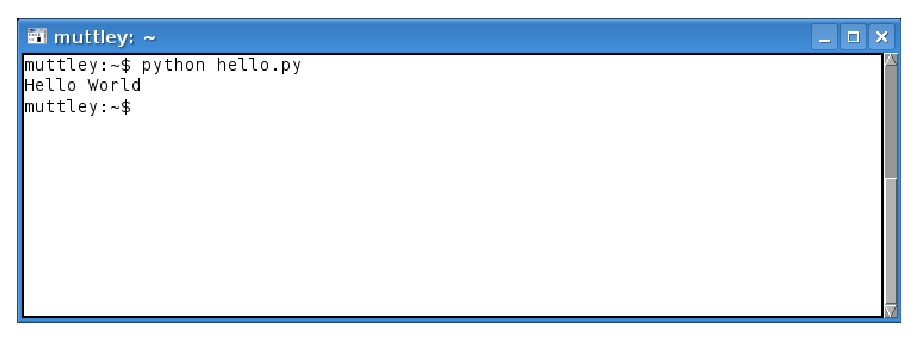
\includegraphics[width=75mm]{figure9.eps}
\end{center}
%\caption{Running a python program from a text file on Linux.}\label{fig9}
\caption{Das Python Programm direkt über ein Textfile aufrufen.}\label{fig9}
\end{figure}
\end{LINUX}

%So you can now see that the nice people who created Python, have kindly saved you from having to type the same thing over and over and over and over and over again.  Like they did back in the 1980's.  No, I'm serious---they did.  Go and ask your Dad if he ever owned a ZX81 when he was younger?\\
Wie du siehst sparst du dir damit die Arbeit die gleichen Dinge immer wieder und wieder einzutippen. So war es in den 1980'er Jahren. Ich mache keine Witze---früher war es so. Geh und frag deinen Vater ob er jemals eine ZX81 verwendet hat, als er jünger war.\\

\noindent
%%If he did you can point at him and laugh.\\
Wenn ja, kannst du mit dem Finger auf ihn zeigen und lachen.\\

\noindent
%Trust me on this one.  You won't get it.  But he will.\footnote{The Sinclair ZX81, released in the 1980's was one of the first affordable home computers.  A number of young boys and girls were driven completely mad, typing in the code for games printed in popular ZX81 magazines---only to discover, after hours of typing, that the darn things never worked properly.}
Bei dem musst du mir vertrauen. Du wirst es nicht verstehen. Aber dein Vater wird. \footnote{Der Sinclair ZX81, der in den 1980'er herauskam, war einer der ersten Computer, die man sich leisten konnte. Viele junge Jungen und Mädchen haben sich halb totgeärgert, als sie den Code aus dem populären ZX81 Magazin abtippten nur um später festzustellen, dass das verdammte Ding überhaupt nie richtig funktionierte.}


\noindent
%\emph{Be prepared to run away though.}
\emph{Sei aber vorbereitet davonzulaufen.}

%\subsection*{\color{BrickRed}The End of the Beginning}
\subsection*{\color{BrickRed}Das Ende des Anfangs}

%Welcome to the wonderful world of Programming.  We've started really simply with a ``Hello World'' application---everyone starts with that, when they're learning to program.
Willkommen in der wunderbaren welt der Programmierung. Wir haben ganz einfach angefangen mit einem ``Hallo Welt'' Programm---jeder fängt mit diesem an wenn man programmieren lernt.
%In the next chapter we'll start to do some more useful things with the Python console and then look at what goes into making a program.
Im nächsten Kapitel werden wir anfangen einige etwas sinnvollere Dinge mit der Python Konsole zu machen und lernen wie man Programme aufbaut.

\newpage
